\section{Linear classification and logistic regression}
\label{sec:linear-classification-and-logistic-regression}

\subsection{Purpose of this stage}

This stage introduces the first learned classification models in the project. The previous stages established the statistical evaluation methodology, the binary classification evaluation framework, simple dummy baselines, and an EDA-inspired rule. The purpose here is to move from manually specified or non-informative baselines to learned linear classifiers that estimate decision rules from the training data.

The held-out test set is not used in this section. All performance estimates are based on stratified cross-validation inside the training set. Preprocessing is included inside each modelling pipeline, so scaling and one-hot encoding are fitted only on the training portion of each cross-validation fold.

The models considered in this section are regularized least-squares classification, logistic regression with L2 regularization, logistic regression with L1 regularization, and a class-weighted logistic regression variant. These models are useful first learned models because they are mathematically transparent, computationally efficient, and interpretable through their fitted coefficients.

The results in this section should be read as development-stage cross-validated estimates. They are used to understand the behaviour of linear classifiers and to choose representative linear candidates for later comparison. They are not final test-set estimates, and small differences between neighbouring regularization settings should not be interpreted as proof of unique population-level optimality.

\subsection{Linear score functions and decision boundaries}

A linear classifier begins with a real-valued score
\[
f(x) = w^\top x + b,
\]
where \(x \in \mathbb{R}^p\) is a feature vector, \(w \in \mathbb{R}^p\) is a vector of weights, and \(b \in \mathbb{R}\) is an intercept. The score is positive on one side of the decision boundary and negative on the other side.

The decision boundary is the set of feature values for which the score equals zero:
\[
w^\top x + b = 0.
\]
In two dimensions this boundary is a line, in three dimensions it is a plane, and in higher dimensions it is a hyperplane. A simple binary prediction rule is
\[
\hat{y}
=
\begin{cases}
1, & f(x) \geq 0,\\
0, & f(x) < 0.
\end{cases}
\]
In this project, \(1\) denotes churn and \(0\) denotes no churn. Therefore, a positive score assigns a customer to the churn side of the fitted linear boundary.

Linear classifiers are limited because they are additive in the transformed feature representation. After one-hot encoding, they can learn separate contributions from contract type, internet service, billing, and numeric variables, but they do not automatically learn complex interactions unless those interactions are explicitly added as features. This limitation is useful to remember when later comparing linear models with trees, ensembles, and neural networks.

\subsection{Least-squares classification}

Least-squares classification treats classification as a regression-like problem. If labels are encoded as \(y_i^\star \in \{-1,+1\}\), the fitted score is obtained by minimizing
\[
\min_{w,b}
\sum_{i=1}^n
\left(
w^\top x_i + b - y_i^\star
\right)^2.
\]
In matrix form, with the intercept included in the design matrix, this is
\[
\min_\beta \|X\beta - y^\star\|_2^2.
\]
A regularized version adds an L2 penalty:
\[
\min_\beta \|X\beta - y^\star\|_2^2 + \alpha \|\beta\|_2^2.
\]
This is the idea behind the \texttt{RidgeClassifier} used in this section. It provides a linear classification baseline connected to least-squares learning, while the ridge penalty stabilizes fitting after one-hot encoding.

Least-squares classification is not a probability model. It can produce a useful linear score, but it does not directly model \(P(Y=1 \mid X=x)\). Logistic regression is more appropriate when probability estimates and threshold analysis are needed.

\subsection{Logistic regression}

Logistic regression uses the same linear score,
\[
z_i = w^\top x_i + b,
\]
but maps it to a probability through the sigmoid function:
\[
\sigma(z)
=
\frac{1}{1+\exp(-z)}.
\]
The fitted churn probability is
\[
\hat{p}_i
=
P(Y_i=1\mid X_i=x_i)
=
\sigma(w^\top x_i+b).
\]
The default class prediction uses threshold \(0.5\):
\[
\hat{y}_i
=
\mathbb{1}\{\hat{p}_i \geq 0.5\}.
\]
Because the sigmoid is monotonic and \(\sigma(0)=0.5\), this default threshold corresponds to the linear boundary \(w^\top x+b=0\).

Logistic regression can also be written as a log-odds model:
\[
\log\left(\frac{p(x)}{1-p(x)}\right)
=
w^\top x+b.
\]
A coefficient \(w_j\) is therefore a change in log-odds associated with a one-unit increase in the transformed feature \(x_j\), holding other transformed features fixed. The odds ratio is
\[
\exp(w_j).
\]
For standardized numeric variables, a one-unit change corresponds to a one-standard-deviation increase in the original numeric feature. For one-hot encoded variables, coefficients describe the contribution of the corresponding category indicator within the fitted linear model. These are fitted associations, not causal effects.

\subsection{Likelihood and log loss}

For binary outcomes, logistic regression assumes
\[
Y_i \mid X_i=x_i \sim \operatorname{Bernoulli}(\hat{p}_i).
\]
The probability of observing \(y_i\) is
\[
P(Y_i=y_i\mid x_i)
=
\hat{p}_i^{y_i}
(1-\hat{p}_i)^{1-y_i}.
\]
The log-likelihood is
\[
\ell(w,b)
=
\sum_{i=1}^n
\left[
y_i\log(\hat{p}_i)
+
(1-y_i)\log(1-\hat{p}_i)
\right].
\]
Equivalently, logistic regression minimizes the negative log-likelihood,
\[
\mathcal{L}(w,b)
=
-
\sum_{i=1}^n
\left[
y_i\log(\hat{p}_i)
+
(1-y_i)\log(1-\hat{p}_i)
\right],
\]
also called binary cross-entropy or log loss. This loss strongly penalizes confident wrong predictions. For example, assigning a very low probability to a true churner gives a large loss contribution.

\subsection{Regularization}

Regularization controls model complexity by penalizing large coefficients. L2-regularized logistic regression minimizes
\[
\mathcal{L}_{L2}(w,b)
=
\mathcal{L}(w,b) + \lambda \|w\|_2^2,
\]
where
\[
\|w\|_2^2 = \sum_{j=1}^p w_j^2.
\]
L2 regularization shrinks coefficients toward zero but usually does not set them exactly to zero.

L1-regularized logistic regression minimizes
\[
\mathcal{L}_{L1}(w,b)
=
\mathcal{L}(w,b) + \lambda \|w\|_1,
\]
where
\[
\|w\|_1 = \sum_{j=1}^p |w_j|.
\]
L1 regularization can set coefficients exactly to zero, making it useful for sparse linear models and feature selection.

In scikit-learn, logistic regression uses \(C\) as inverse regularization strength. Smaller \(C\) means stronger regularization, while larger \(C\) means weaker regularization:
\[
C \propto \frac{1}{\lambda}.
\]
For this first learned-model section, a small log-scale grid is sufficient and more transparent than automated hyperparameter optimization.

\subsection{Model comparison}

Table~\ref{tab:linear-model-comparison} reports the cross-validated performance of the main linear classifiers. Logistic regression with L1 and L2 regularization performs almost identically. The L1 model obtains the highest PR-AUC, approximately \(0.659\), while the L2 model obtains ROC-AUC approximately \(0.846\) and PR-AUC approximately \(0.658\). The class-weighted L2 logistic regression has a much higher recall, approximately \(0.801\), but lower precision, approximately \(0.517\). This is expected because class weighting makes the model more willing to predict the minority churn class.

The L1 and L2 PR-AUC values differ by only about \(0.001\). This is much smaller than the kind of difference that should be interpreted as strong statistical evidence. The practical conclusion is that both L1 and L2 logistic regression are competitive in this development-stage comparison. L2 logistic regression is retained as the main coefficient-interpretation model because it is stable, standard, and produces dense coefficients, while L1 remains useful as a sparse alternative.

\begin{table}[H]
\centering
\small
\begin{tabular}{lrrrrrrrr}
\toprule
Model & Acc. & Bal. acc. & Prec. & Recall & Spec. & F1 & ROC-AUC & PR-AUC \\
\midrule
Logistic L1 C=1 & 0.802 & 0.720 & 0.654 & 0.543 & 0.896 & 0.593 & 0.846 & 0.659 \\
Logistic L2 C=1 & 0.802 & 0.719 & 0.652 & 0.544 & 0.895 & 0.593 & 0.846 & 0.658 \\
Logistic L2 balanced C=1 & 0.748 & 0.765 & 0.517 & 0.801 & 0.729 & 0.628 & 0.846 & 0.657 \\
RidgeClassifier alpha=1 & 0.801 & 0.712 & 0.659 & 0.521 & 0.903 & 0.582 & 0.838 & 0.649 \\
\bottomrule
\end{tabular}
\caption{Cross-validated linear-model comparison on the training set.}
\label{tab:linear-model-comparison}
\end{table}

The confusion-matrix counts in Table~\ref{tab:linear-confusion} clarify the tradeoff. The standard L2 logistic regression detects \(813\) churners and misses \(682\). The class-weighted variant detects \(1198\) churners but increases false positives from \(434\) to \(1120\). Therefore, class weighting improves recall but does so by flagging many more non-churners.

\begin{table}[H]
\centering
\begin{tabular}{lrrrr}
\toprule
Model & TP & FN & FP & TN \\
\midrule
Logistic L1 C=1 & 812 & 683 & 430 & 3709 \\
Logistic L2 C=1 & 813 & 682 & 434 & 3705 \\
Logistic L2 balanced C=1 & 1198 & 297 & 1120 & 3019 \\
RidgeClassifier alpha=1 & 779 & 716 & 403 & 3736 \\
\bottomrule
\end{tabular}
\caption{Cross-validated confusion-matrix counts in positive-first order.}
\label{tab:linear-confusion}
\end{table}

\subsection{Regularization results}

Table~\ref{tab:l2-regularization} and Figure~\ref{fig:l2-regularization} show the L2 regularization path. Very strong regularization, \(C=0.001\), produces a conservative classifier with high precision but low recall. As \(C\) increases, recall and F1 improve. The ranking metrics are stable over most of the grid, with ROC-AUC around \(0.845\) and PR-AUC around \(0.658\) once \(C\geq 0.1\). This indicates that the logistic model is not highly sensitive to the exact L2 regularization strength over the tested range.

This is a good example of why the report should focus on stable hyperparameter regions rather than exact winners. The difference between \(C=0.1\), \(C=1\), \(C=10\), and \(C=100\) is very small for ROC-AUC and PR-AUC. The development-stage evidence mainly says that extremely strong L2 regularization underfits, while a broad range of weaker regularization strengths performs similarly.

\begin{table}[H]
\centering
\small
\begin{tabular}{rrrrrrrr}
\toprule
\(C\) & Acc. & Bal. acc. & Prec. & Recall & F1 & ROC-AUC & PR-AUC \\
\midrule
0.001 & 0.777 & 0.599 & 0.780 & 0.220 & 0.343 & 0.839 & 0.651 \\
0.01 & 0.805 & 0.711 & 0.674 & 0.511 & 0.581 & 0.843 & 0.656 \\
0.1 & 0.801 & 0.717 & 0.652 & 0.538 & 0.590 & 0.845 & 0.658 \\
1 & 0.802 & 0.719 & 0.652 & 0.544 & 0.593 & 0.846 & 0.658 \\
10 & 0.804 & 0.723 & 0.656 & 0.549 & 0.598 & 0.846 & 0.658 \\
100 & 0.804 & 0.723 & 0.655 & 0.550 & 0.598 & 0.846 & 0.657 \\
\bottomrule
\end{tabular}
\caption{L2 logistic regression regularization grid.}
\label{tab:l2-regularization}
\end{table}

\begin{figure}[H]
\centering
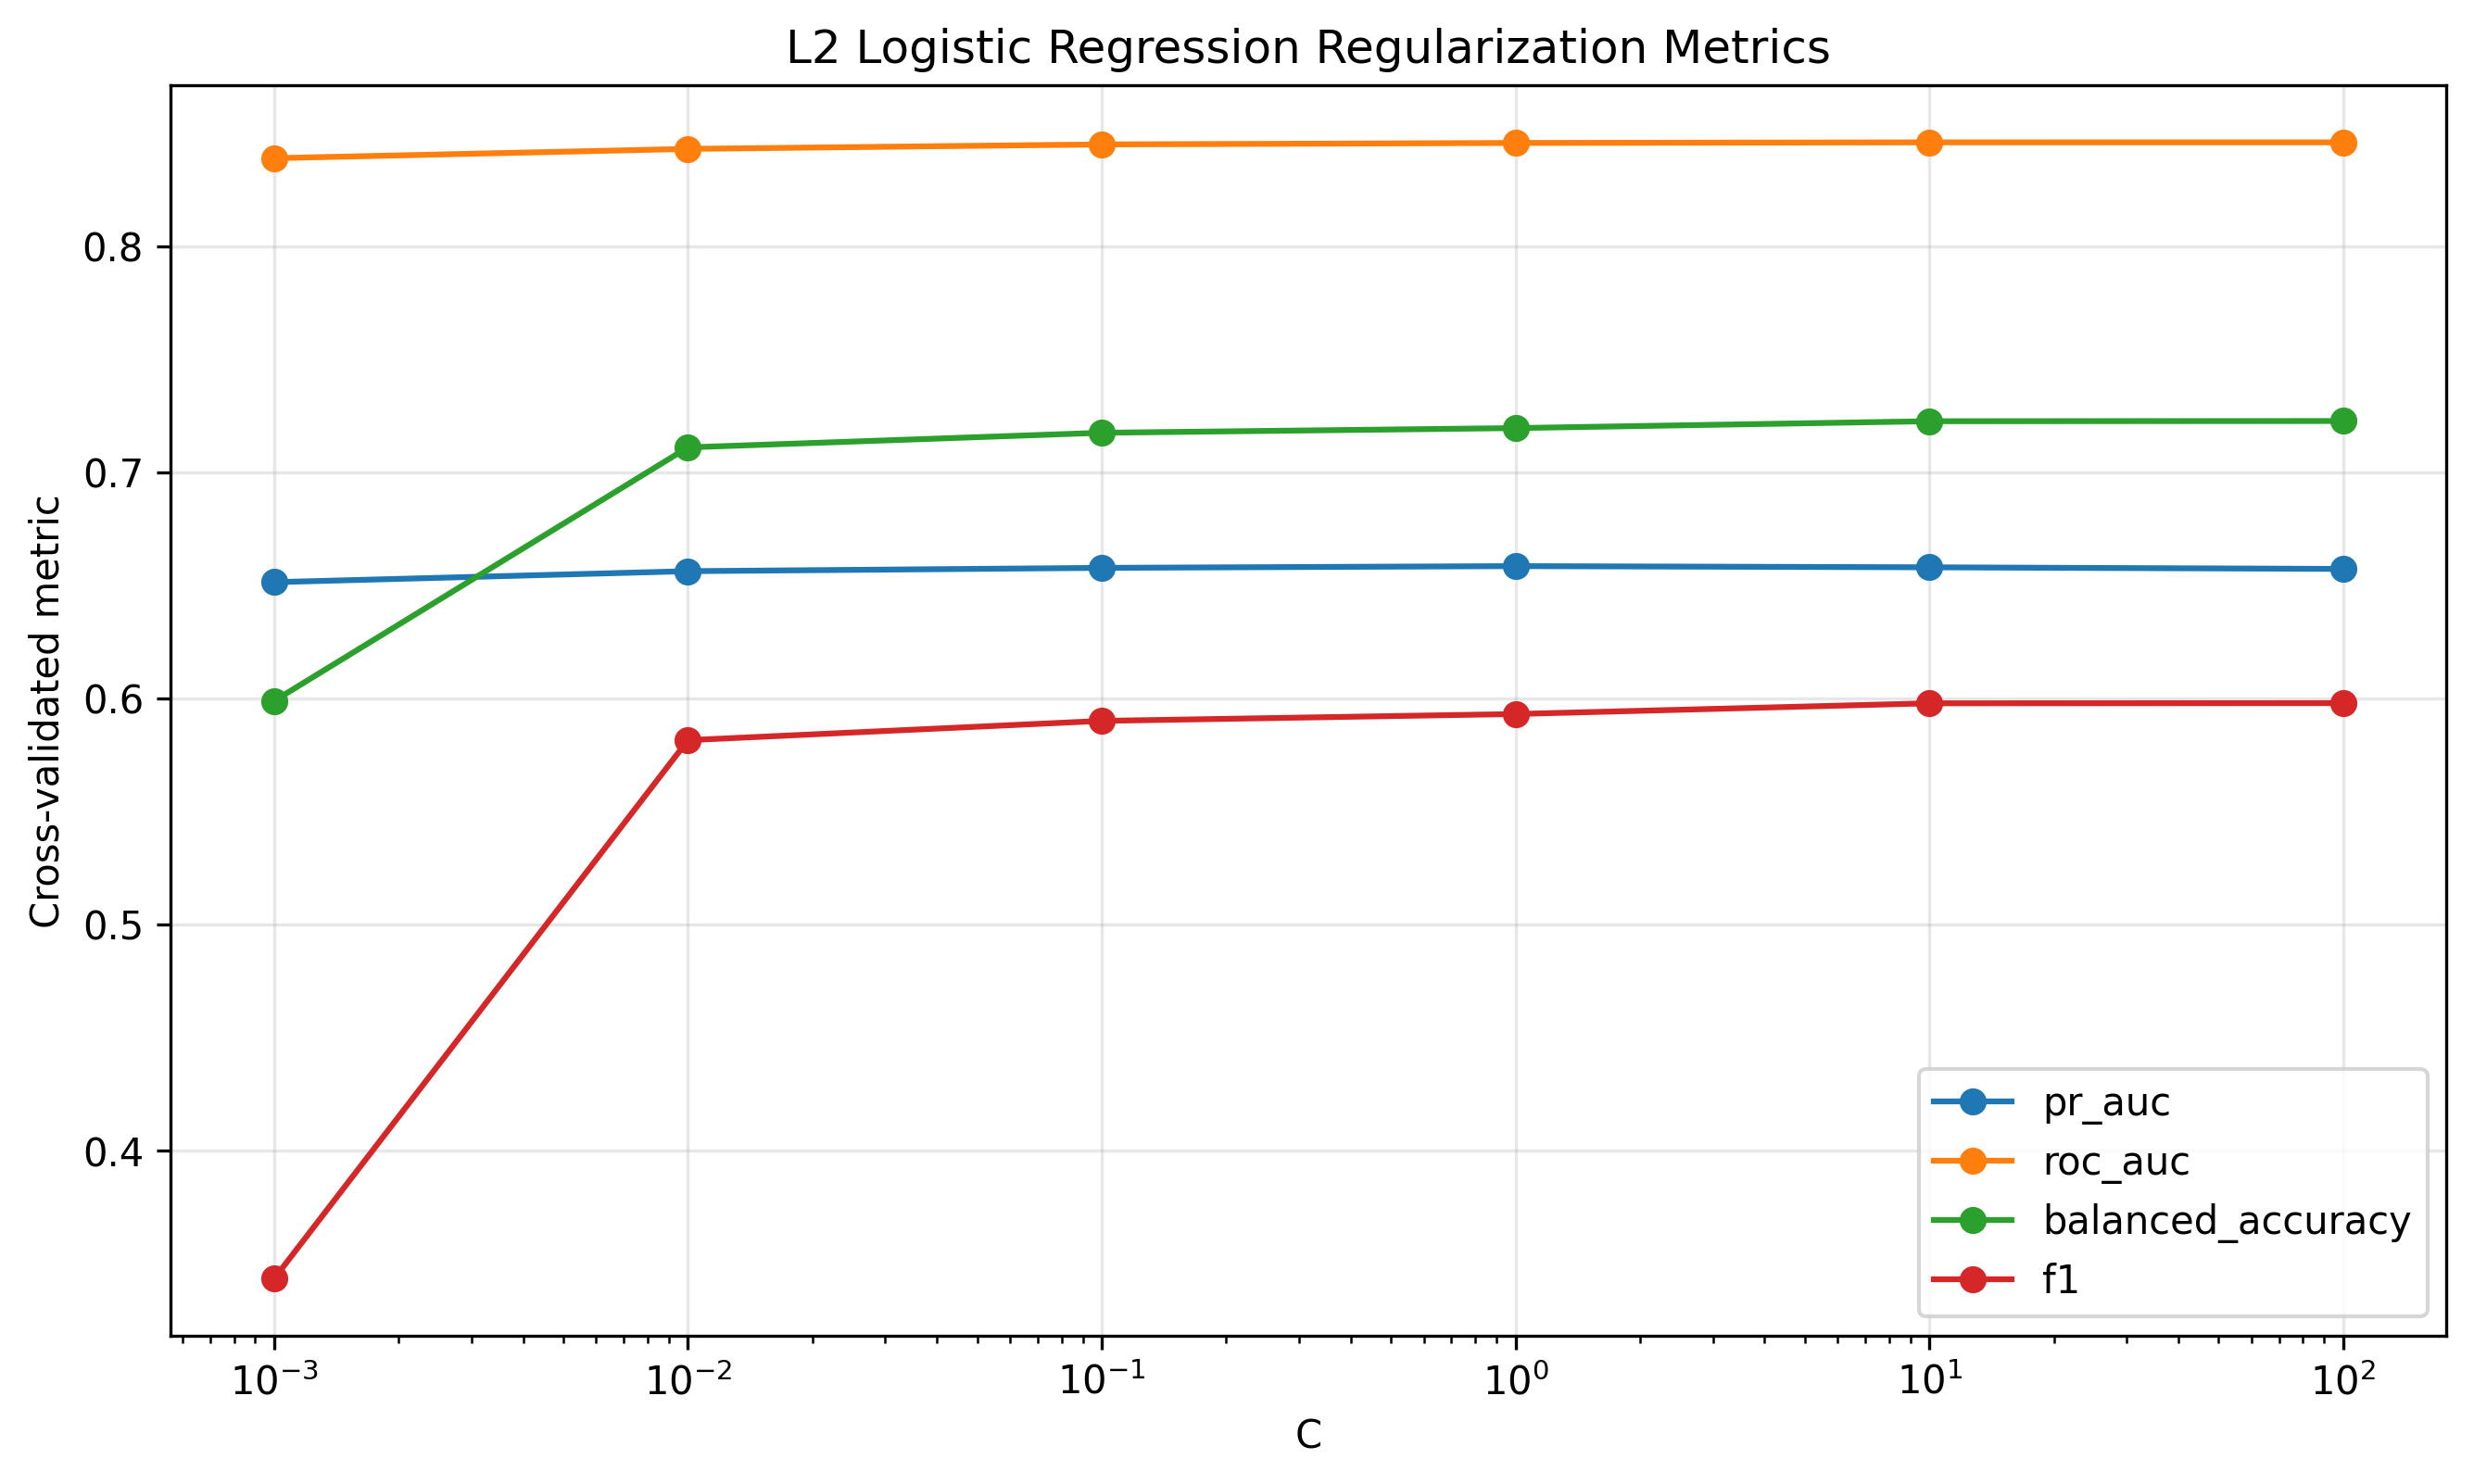
\includegraphics[width=0.82\textwidth]{../figures/logistic_l2_regularization_metrics.png}
\caption{L2 logistic regression metrics over the regularization grid.}
\label{fig:l2-regularization}
\end{figure}

The L1 grid in Table~\ref{tab:l1-regularization} and Figure~\ref{fig:l1-regularization} shows a more visible effect of very strong regularization. At \(C=0.001\), the L1 model effectively predicts no churners, so recall and F1 are zero and PR-AUC equals the positive-class prevalence. Once \(C\) reaches \(0.1\) or larger, the L1 model behaves similarly to L2 logistic regression. This suggests that mild L1 regularization is compatible with the predictive structure in the data, but excessive sparsity removes too much useful signal.

Here again, the exact best value should not be overinterpreted. \(C=1\) and \(C=10\) differ only slightly. The important conclusion is that the L1 model needs enough flexibility to keep the relevant one-hot and numeric signals active.

\begin{table}[H]
\centering
\small
\begin{tabular}{rrrrrrrr}
\toprule
\(C\) & Acc. & Bal. acc. & Prec. & Recall & F1 & ROC-AUC & PR-AUC \\
\midrule
0.001 & 0.735 & 0.500 & 0.000 & 0.000 & 0.000 & 0.500 & 0.265 \\
0.01 & 0.794 & 0.673 & 0.684 & 0.416 & 0.517 & 0.825 & 0.632 \\
0.1 & 0.801 & 0.714 & 0.655 & 0.528 & 0.585 & 0.844 & 0.658 \\
1 & 0.802 & 0.720 & 0.654 & 0.543 & 0.593 & 0.846 & 0.659 \\
10 & 0.803 & 0.722 & 0.654 & 0.548 & 0.597 & 0.846 & 0.658 \\
\bottomrule
\end{tabular}
\caption{L1 logistic regression regularization grid.}
\label{tab:l1-regularization}
\end{table}

\begin{figure}[H]
\centering
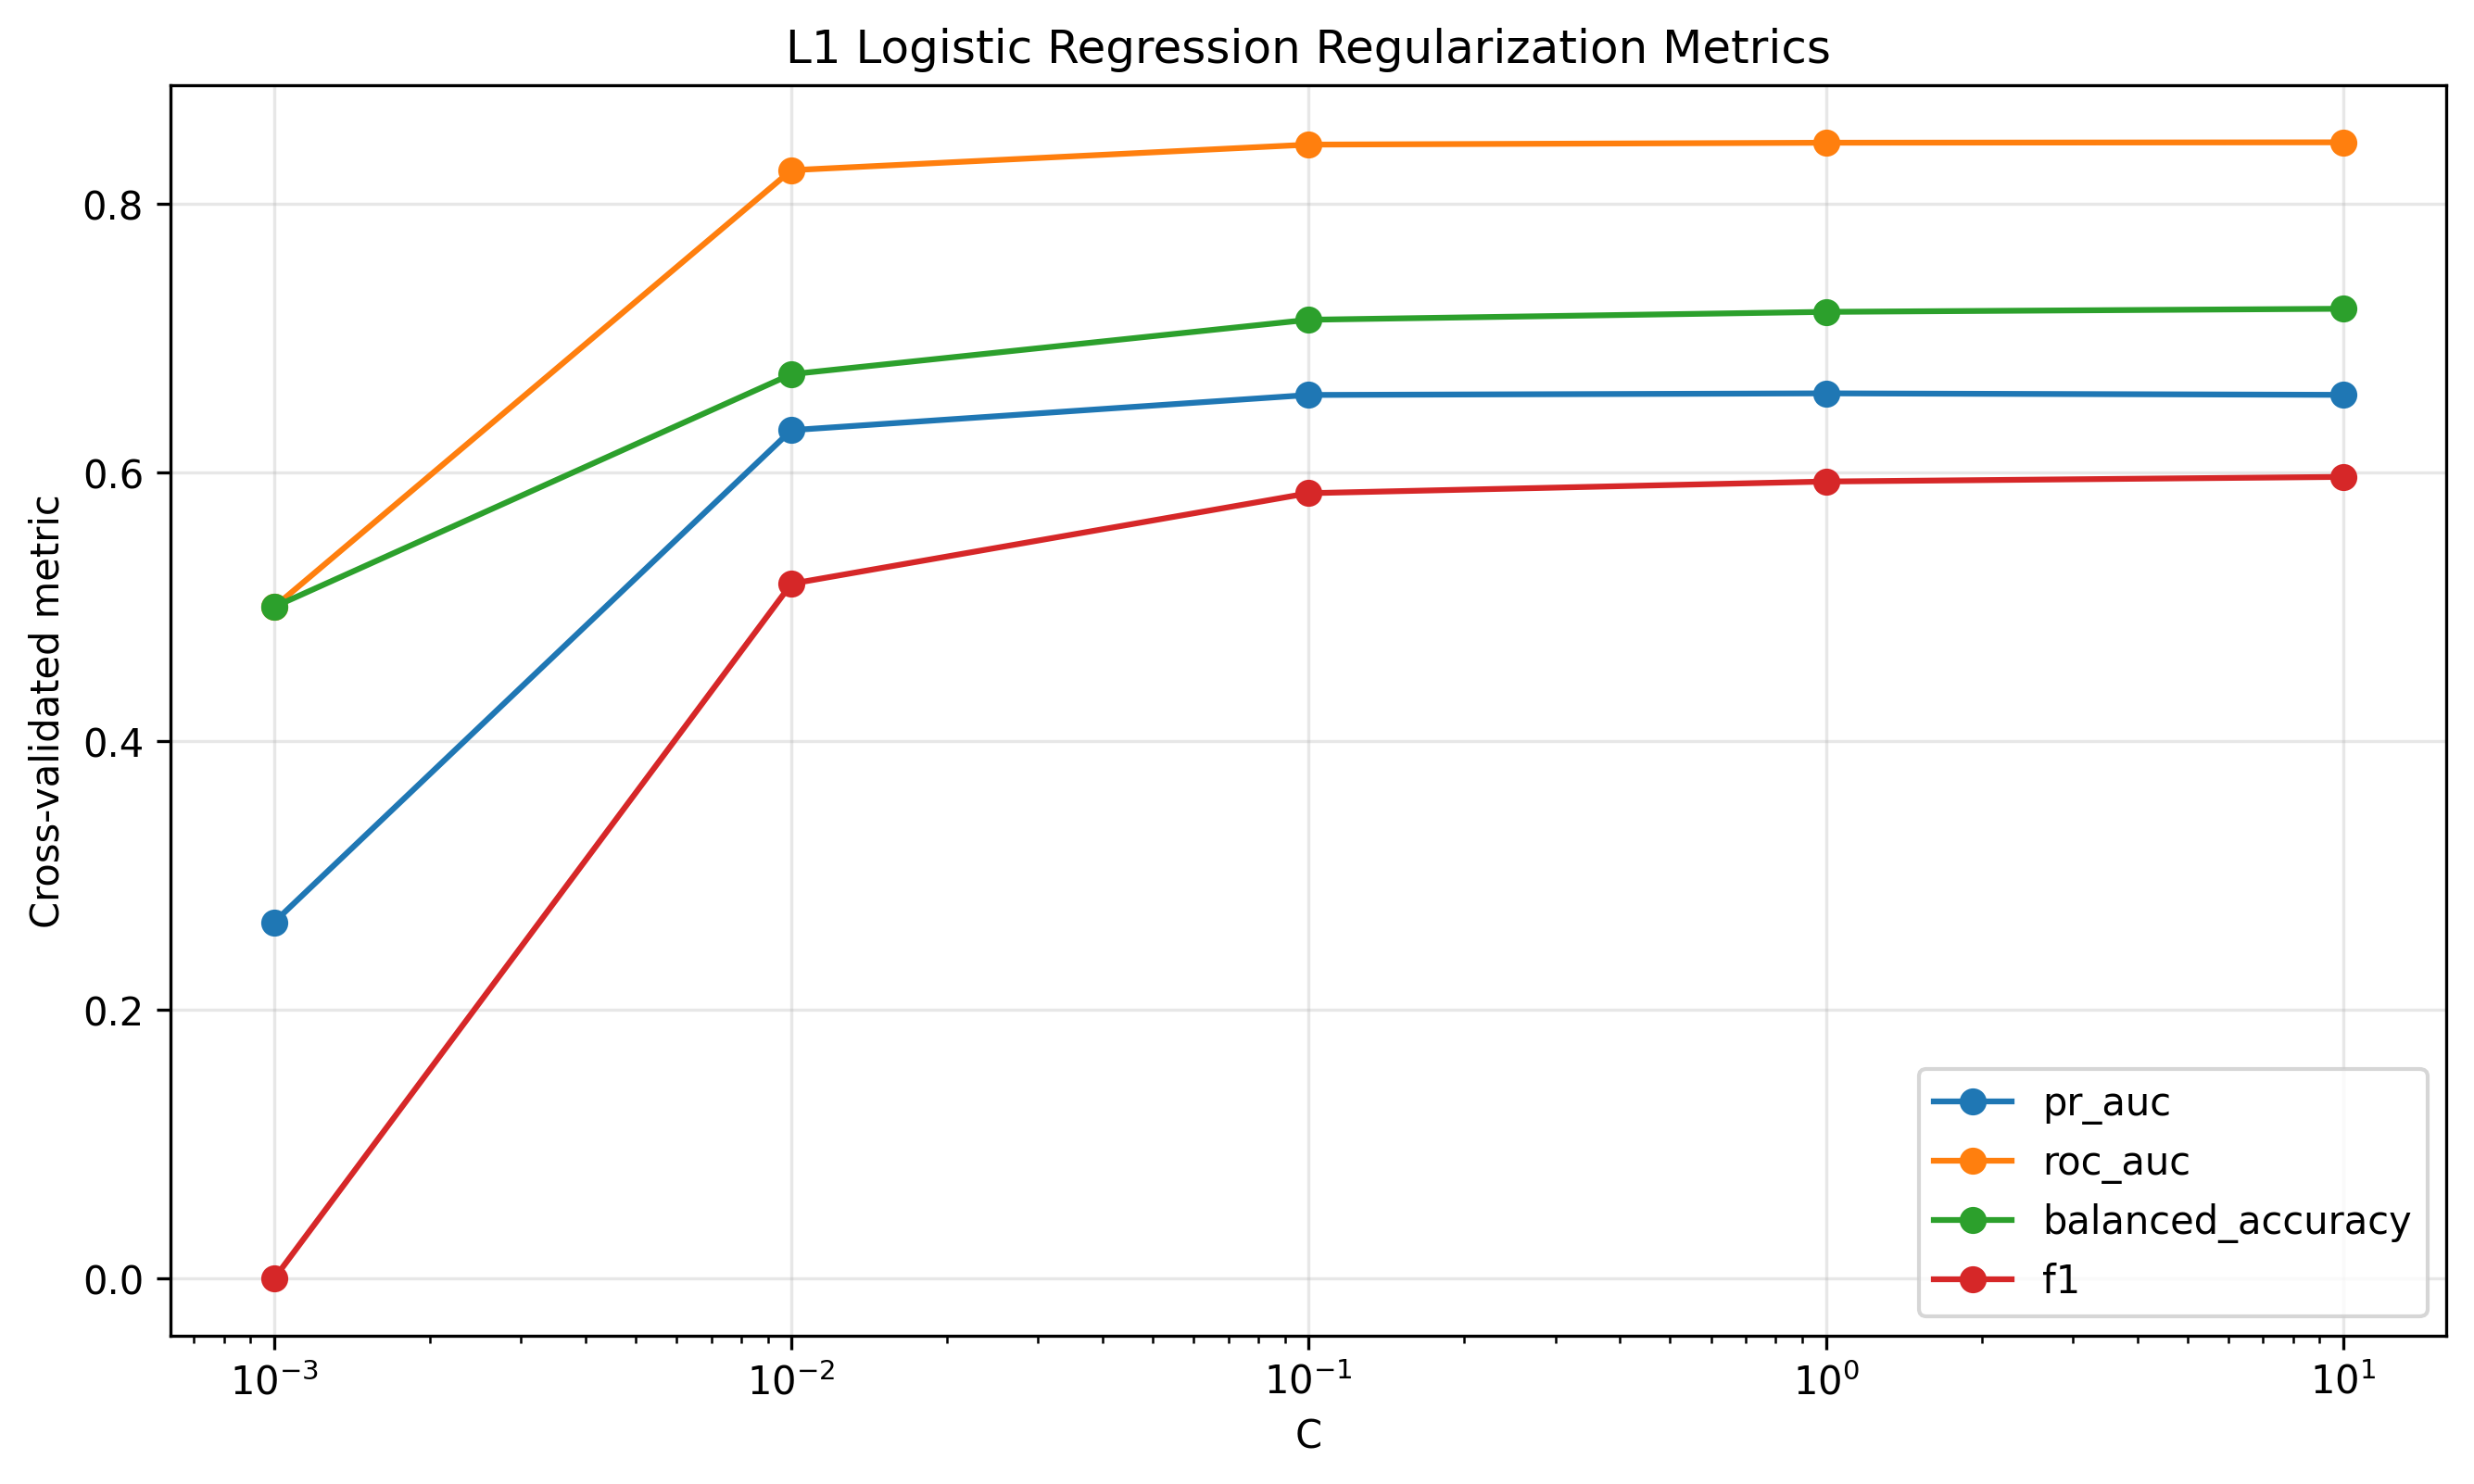
\includegraphics[width=0.82\textwidth]{../figures/logistic_l1_regularization_metrics.png}
\caption{L1 logistic regression metrics over the regularization grid.}
\label{fig:l1-regularization}
\end{figure}

\subsection{Selected logistic model and coefficient interpretation}

For interpretation, the selected model is the L2 logistic regression model with \(C=1\). This is not selected because it is statistically proven to be uniquely optimal. Rather, it is a representative, stable, standard logistic model from the high-performing regularization region. It has development-stage PR-AUC essentially equal to the best L2 configurations, and it supports straightforward coefficient interpretation. The model is fitted on the full training set only for coefficient extraction. These fitted coefficients are not used to report in-sample performance.

Table~\ref{tab:logistic-coefficients} and Figure~\ref{fig:logistic-coefficients} show the largest coefficients by absolute value. The strongest negative coefficient is \texttt{tenure}, meaning longer-tenure customers receive lower fitted churn scores. \texttt{Contract\_Two year} also has a negative coefficient, consistent with the EDA finding that two-year contracts have low churn rates. The strongest positive coefficients are \texttt{InternetService\_Fiber optic}, \texttt{Contract\_Month-to-month}, and \texttt{TotalCharges}, all associated with higher fitted churn scores in this linear model.

A notable pattern is that \texttt{MonthlyCharges} has a negative coefficient while \texttt{TotalCharges} has a positive coefficient. This should not be interpreted in isolation as a simple marginal effect. Logistic regression estimates partial associations after controlling for the other encoded features. Since \texttt{tenure}, \texttt{MonthlyCharges}, and \texttt{TotalCharges} are related, their coefficients reflect a conditional linear decomposition rather than the marginal patterns seen in EDA.

\begin{table}[H]
\centering
\small
\begin{tabular}{lrrl}
\toprule
Feature & Coef. & Odds ratio & Direction \\
\midrule
\texttt{tenure} & -1.255 & 0.285 & lower churn score \\
\texttt{Contract\_Two year} & -0.759 & 0.468 & lower churn score \\
\texttt{InternetService\_Fiber optic} & 0.648 & 1.912 & higher churn score \\
\texttt{InternetService\_DSL} & -0.644 & 0.525 & lower churn score \\
\texttt{MonthlyCharges} & -0.601 & 0.548 & lower churn score \\
\texttt{Contract\_Month-to-month} & 0.586 & 1.797 & higher churn score \\
\texttt{TotalCharges} & 0.533 & 1.703 & higher churn score \\
\texttt{PaperlessBilling\_No} & -0.331 & 0.718 & lower churn score \\
\texttt{DeviceProtection\_No internet service} & -0.293 & 0.746 & lower churn score \\
\texttt{OnlineBackup\_No internet service} & -0.293 & 0.746 & lower churn score \\
\texttt{OnlineSecurity\_No internet service} & -0.293 & 0.746 & lower churn score \\
\texttt{InternetService\_No} & -0.293 & 0.746 & lower churn score \\
\bottomrule
\end{tabular}
\caption{Largest selected logistic regression coefficients by absolute value.}
\label{tab:logistic-coefficients}
\end{table}

\begin{figure}[H]
\centering
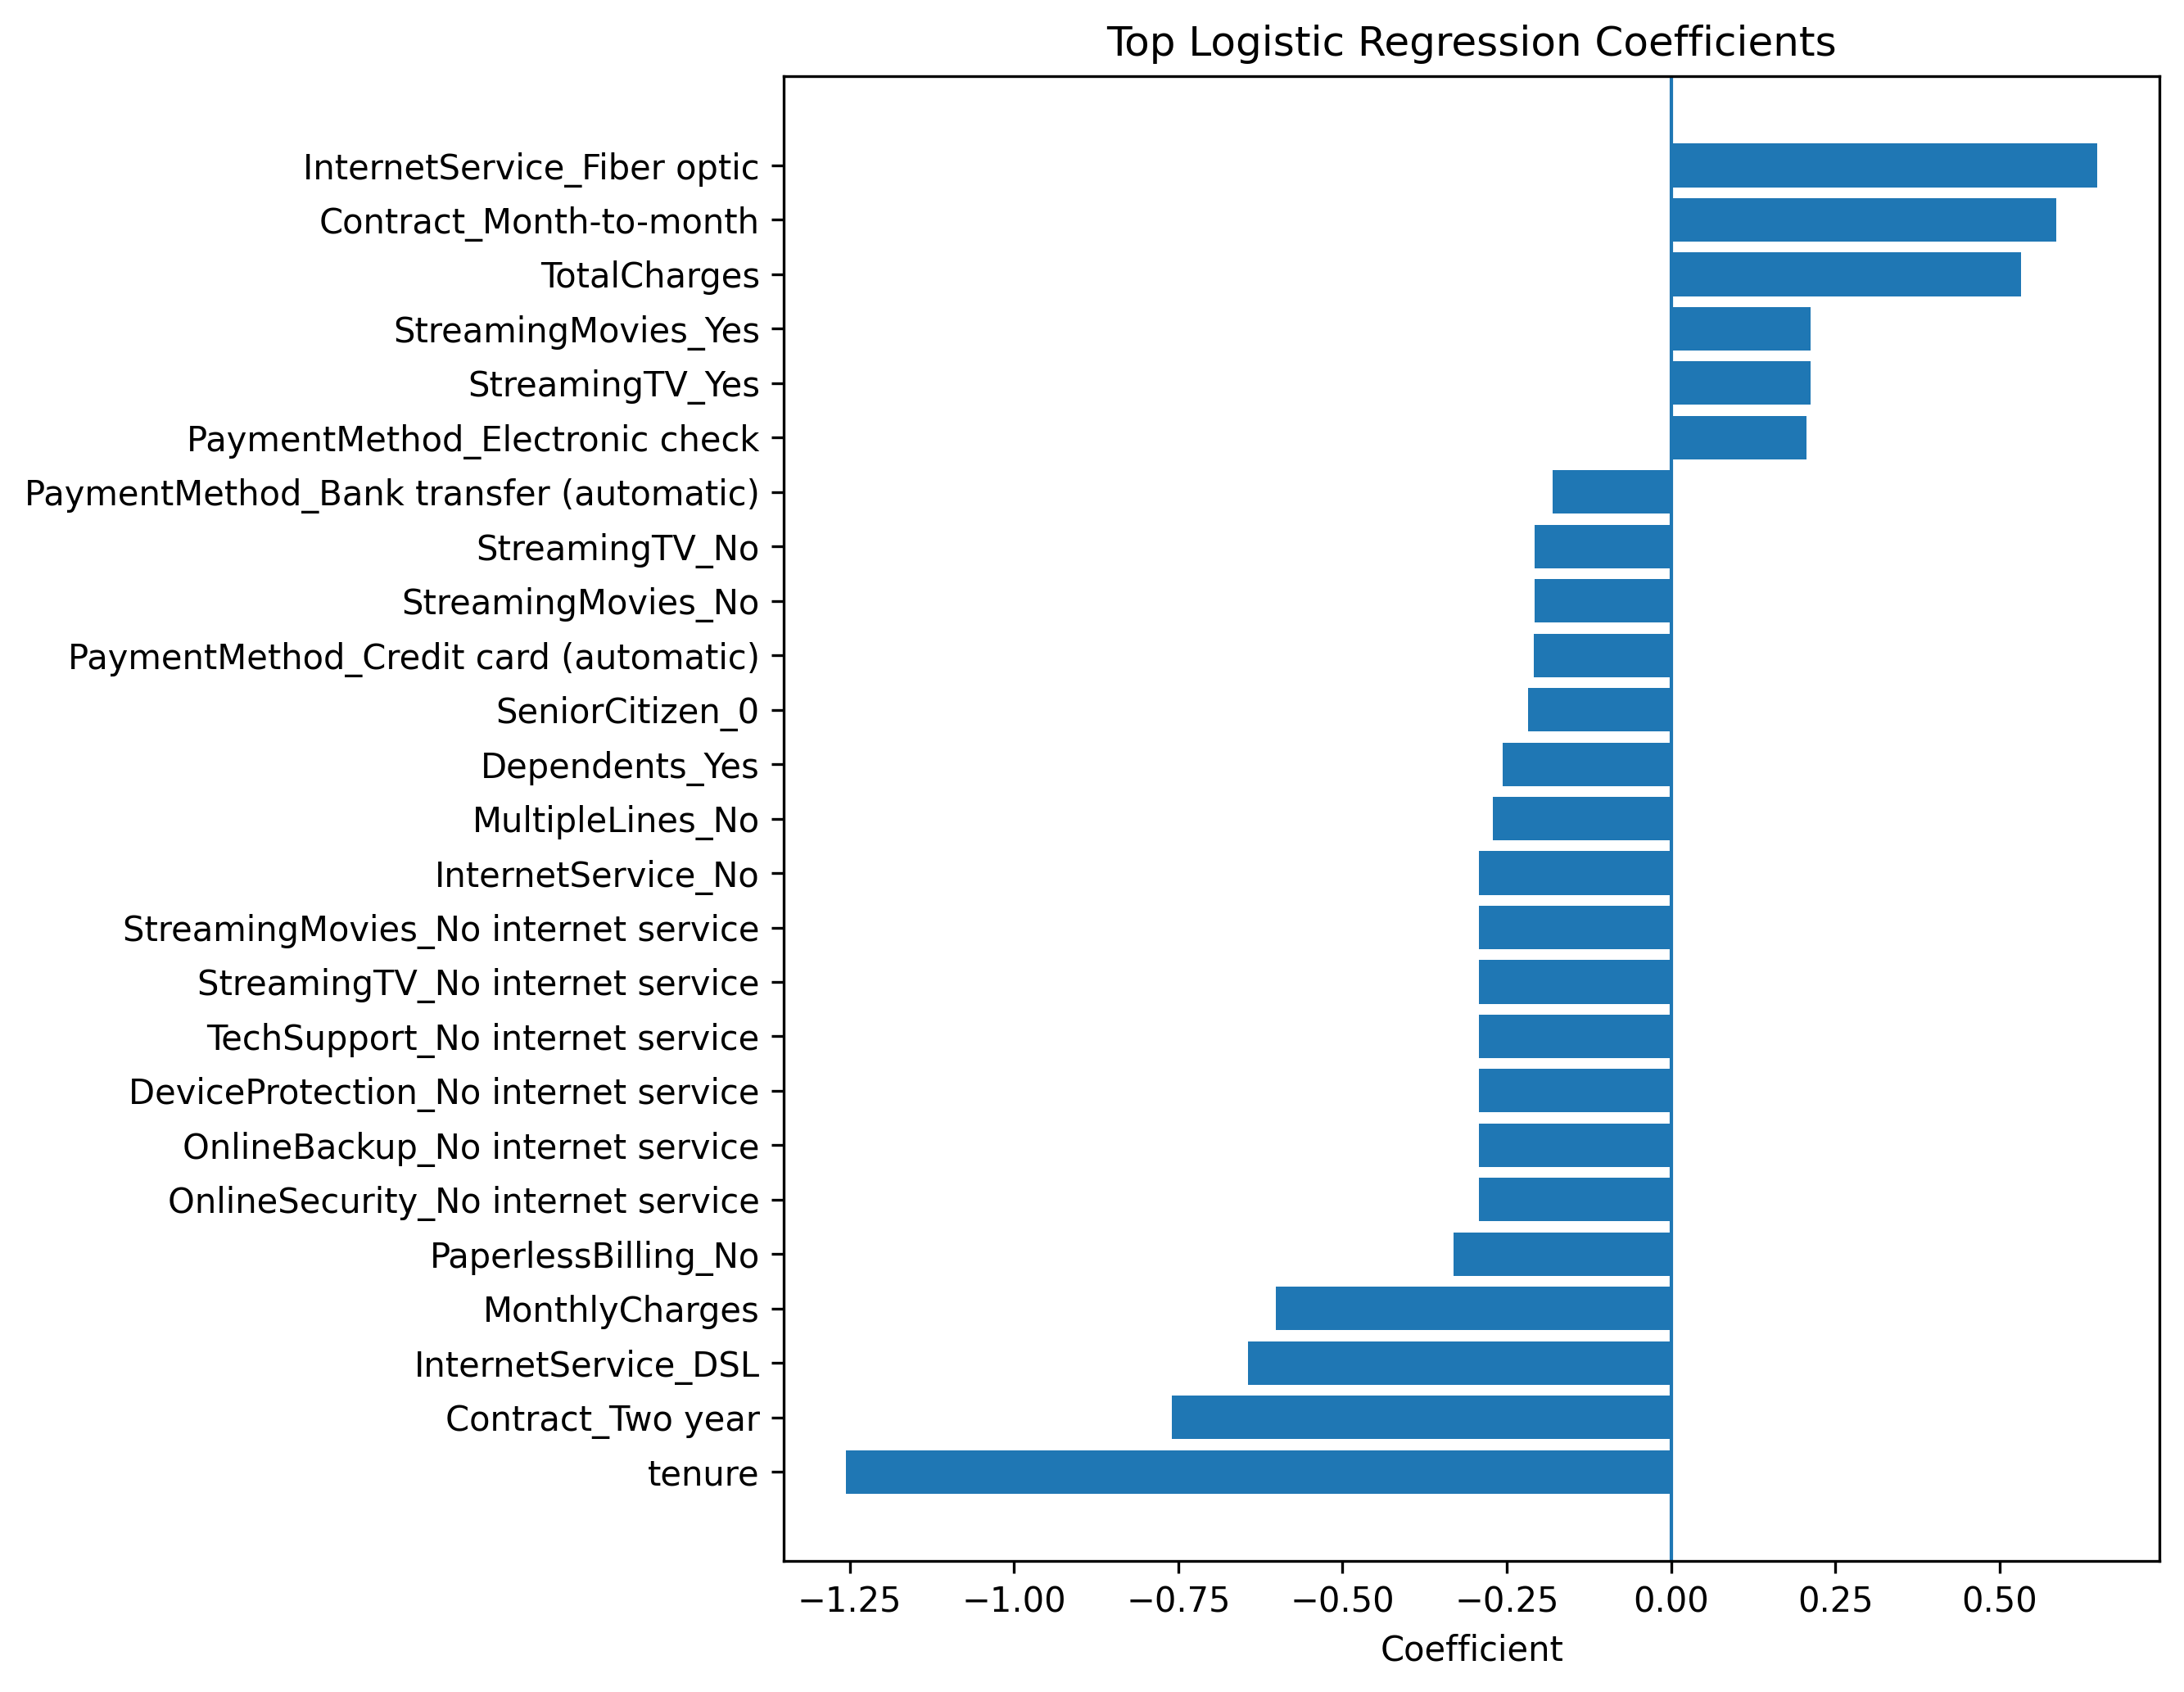
\includegraphics[width=0.82\textwidth]{../figures/logistic_top_coefficients.png}
\caption{Top logistic regression coefficients by absolute magnitude.}
\label{fig:logistic-coefficients}
\end{figure}

\subsection{Threshold tradeoff}

The default logistic regression threshold is \(0.5\), but threshold choice controls the tradeoff between recall, precision, and specificity. Table~\ref{tab:threshold-tradeoff} reports selected thresholds using out-of-fold predicted probabilities. Lowering the threshold increases recall and the predicted positive rate, while raising the threshold increases precision and specificity.

At threshold \(0.50\), the selected L2 logistic model has precision \(0.652\), recall \(0.544\), specificity \(0.895\), and F1 \(0.593\). At threshold \(0.30\), recall increases to \(0.767\), while precision decreases to \(0.541\) and specificity decreases to \(0.765\). The F1 score is highest around thresholds \(0.30\) to \(0.35\) among the displayed values. This does not mean that the final threshold should be chosen here. Final threshold selection should be postponed until model families are compared and the project objective is specified more explicitly.

\begin{table}[H]
\centering
\small
\begin{tabular}{rrrrrrrr}
\toprule
Threshold & Acc. & Bal. acc. & Prec. & Recall & Spec. & F1 & Pred. pos. rate \\
\midrule
0.10 & 0.611 & 0.716 & 0.401 & 0.942 & 0.491 & 0.562 & 0.624 \\
0.20 & 0.711 & 0.757 & 0.475 & 0.854 & 0.659 & 0.610 & 0.477 \\
0.25 & 0.742 & 0.766 & 0.509 & 0.817 & 0.715 & 0.627 & 0.426 \\
0.30 & 0.766 & 0.766 & 0.541 & 0.767 & 0.765 & 0.634 & 0.376 \\
0.35 & 0.782 & 0.761 & 0.571 & 0.717 & 0.805 & 0.635 & 0.334 \\
0.40 & 0.790 & 0.750 & 0.594 & 0.664 & 0.836 & 0.627 & 0.297 \\
0.50 & 0.802 & 0.719 & 0.652 & 0.544 & 0.895 & 0.593 & 0.221 \\
0.60 & 0.797 & 0.669 & 0.710 & 0.397 & 0.942 & 0.509 & 0.148 \\
0.70 & 0.775 & 0.594 & 0.779 & 0.210 & 0.978 & 0.331 & 0.072 \\
\bottomrule
\end{tabular}
\caption{Threshold tradeoff for selected L2 logistic regression using out-of-fold probabilities.}
\label{tab:threshold-tradeoff}
\end{table}

\begin{figure}[H]
\centering
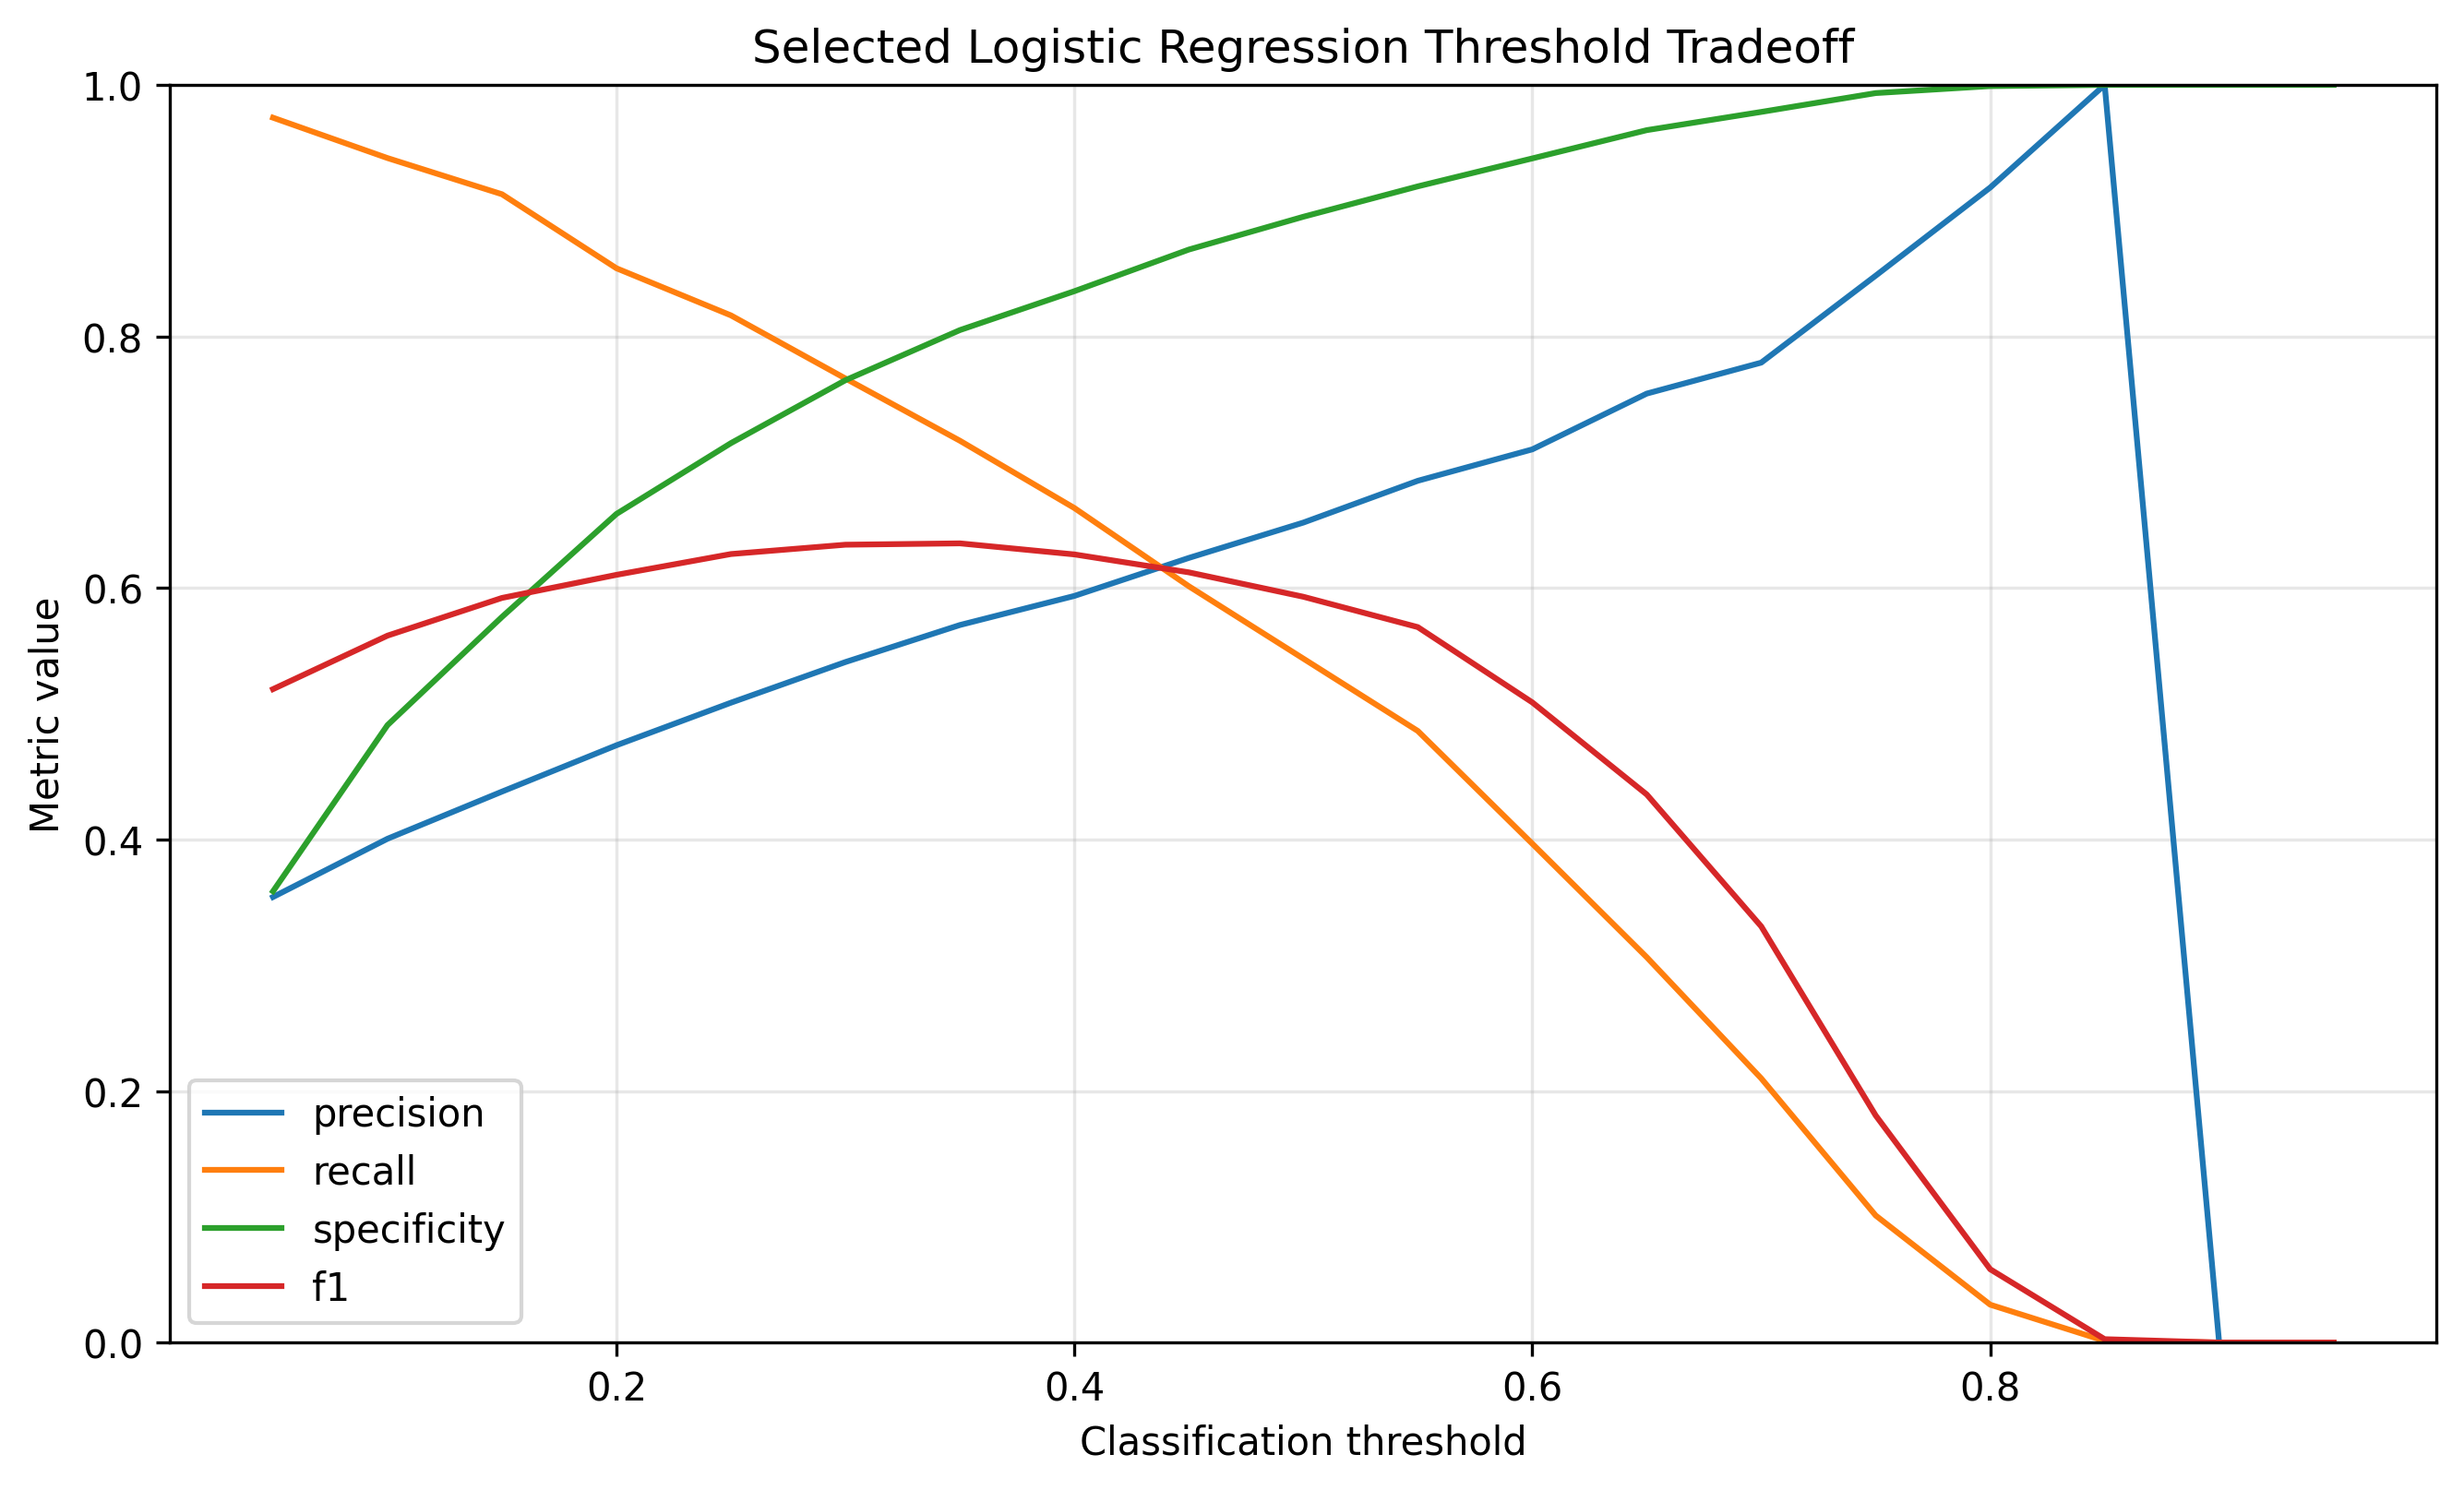
\includegraphics[width=0.82\textwidth]{../figures/logistic_threshold_tradeoff.png}
\caption{Threshold tradeoff for selected L2 logistic regression.}
\label{fig:threshold-tradeoff}
\end{figure}

\subsection{ROC and precision-recall curves}

Figures~\ref{fig:logistic-roc} and~\ref{fig:logistic-pr} summarize threshold-independent ranking performance for the selected logistic regression model. The ROC curve has AUC approximately \(0.846\), indicating that the model ranks churners above non-churners substantially better than a random ranking. The precision-recall curve has AUC approximately \(0.658\), compared with a positive-rate baseline of approximately \(0.265\). This is important because churn is the minority class, and PR-AUC focuses directly on the quality of positive churn retrieval.

\begin{figure}[H]
\centering
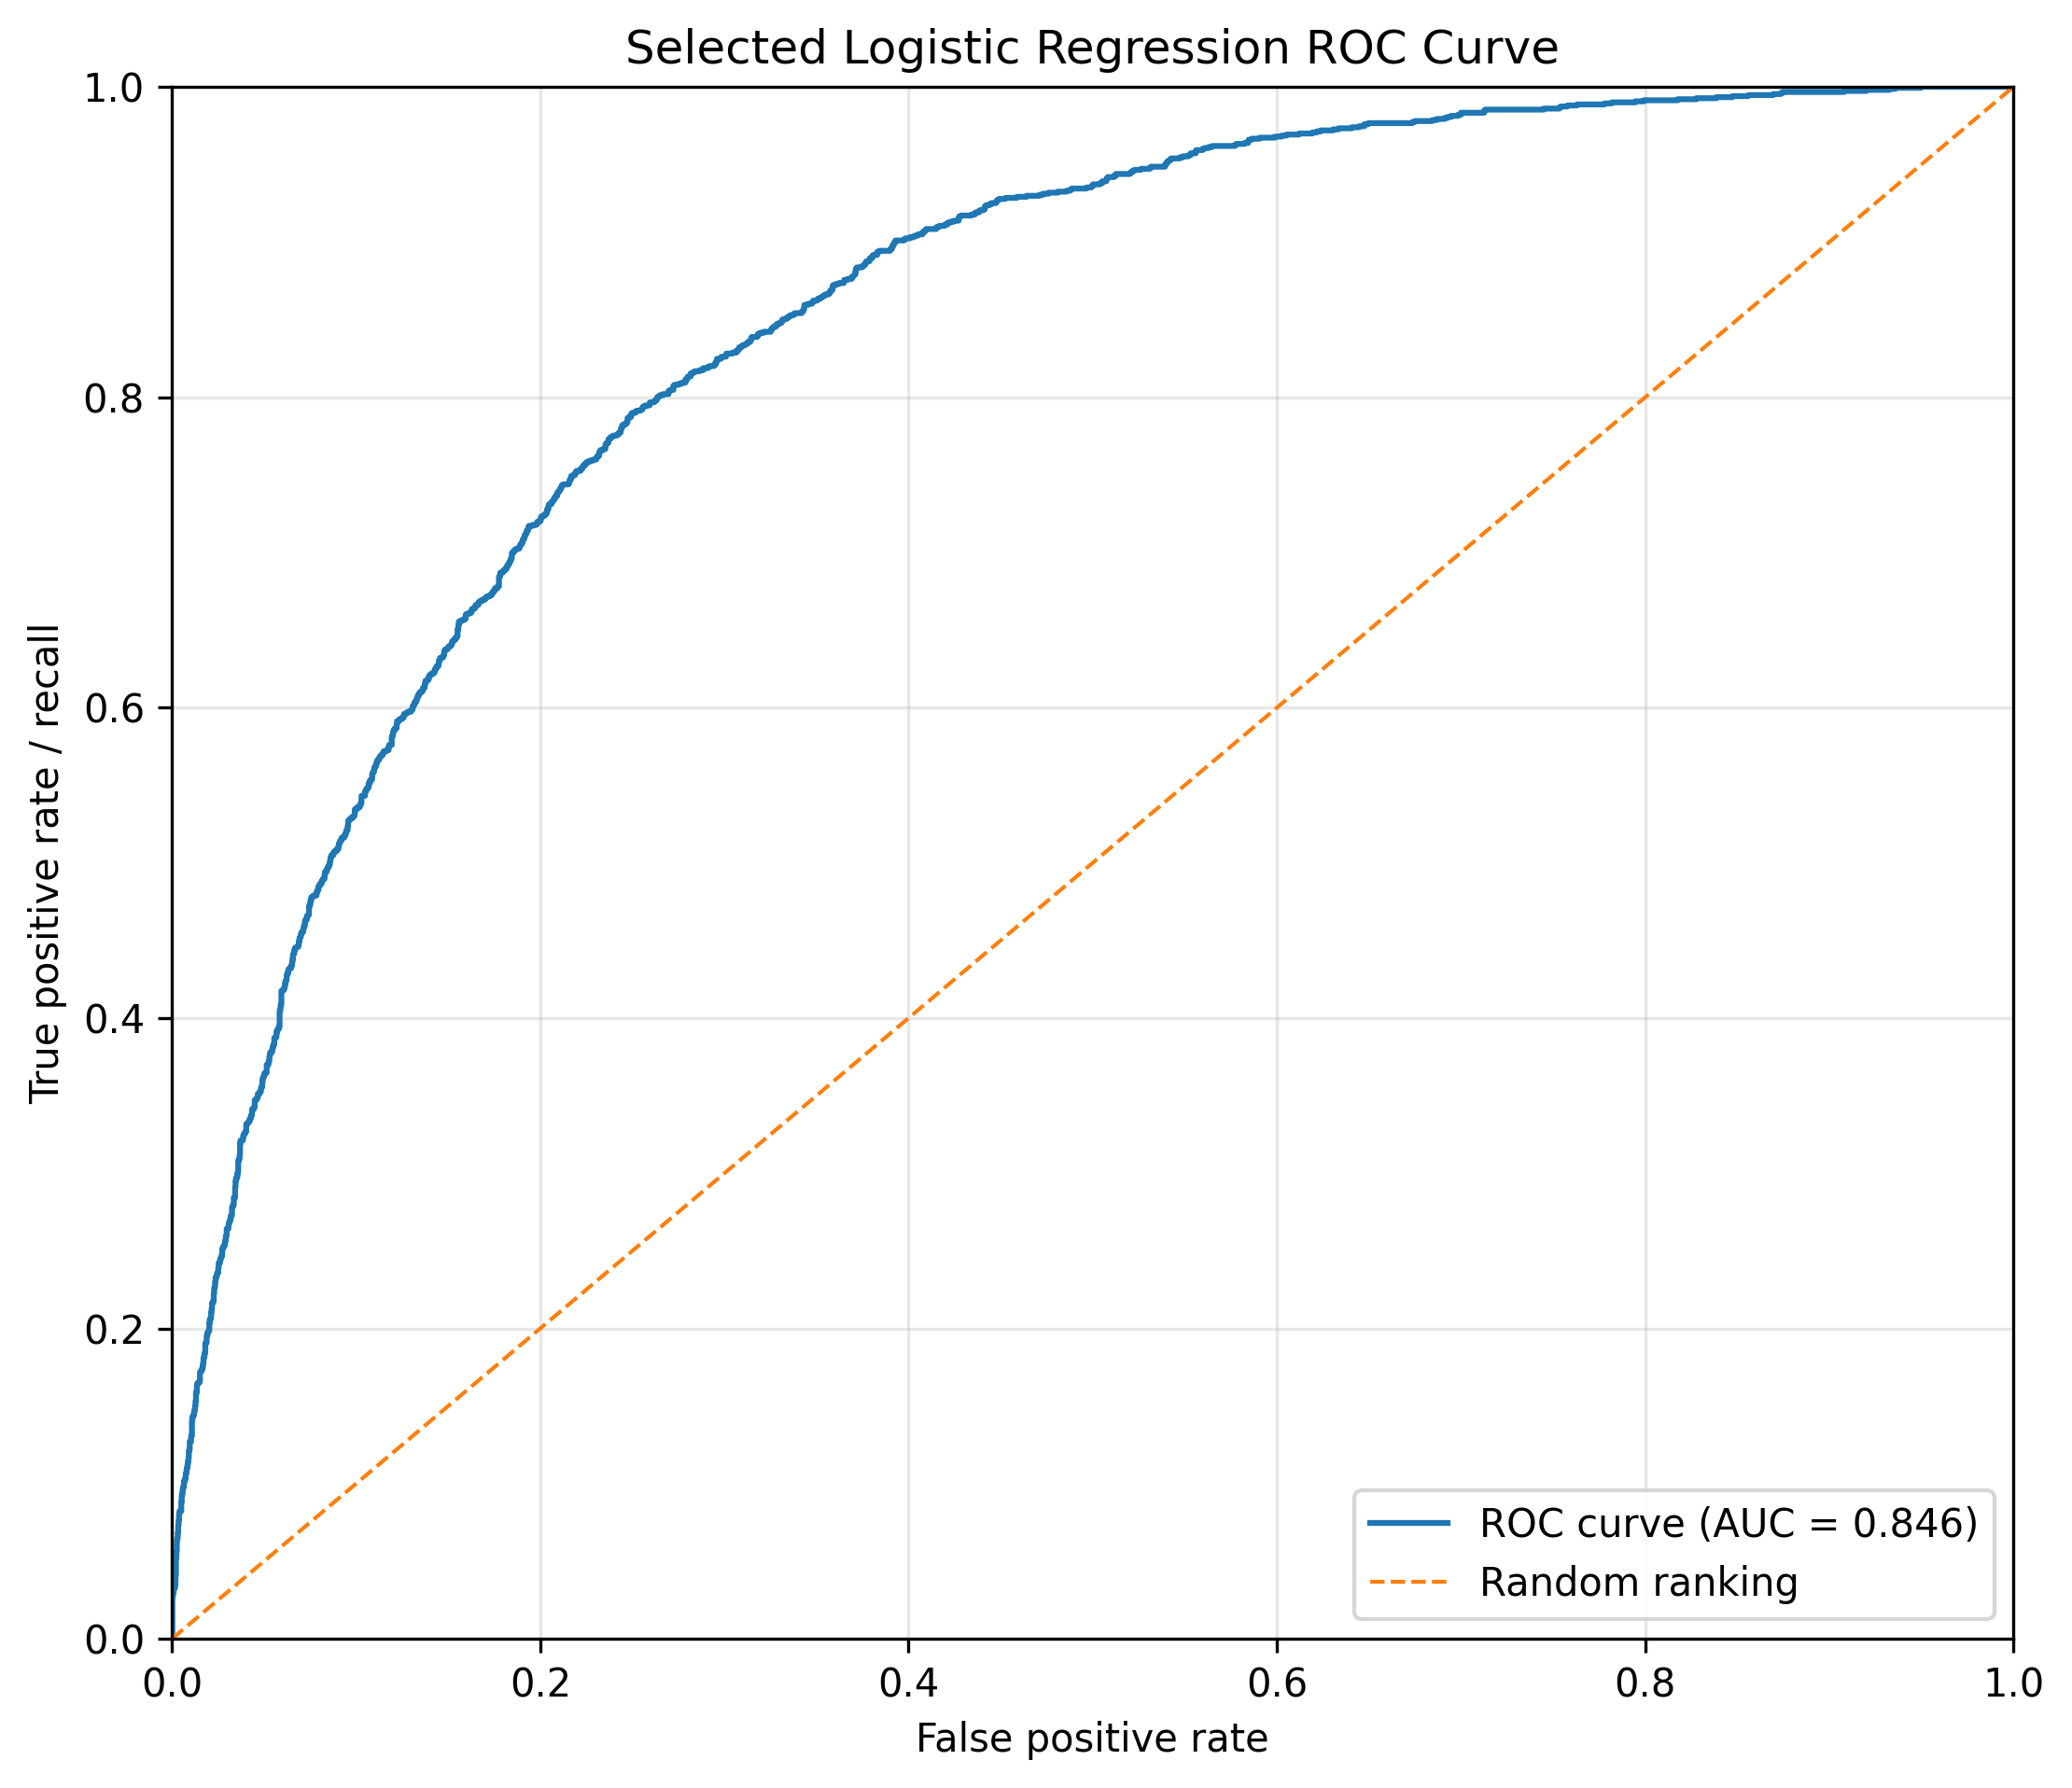
\includegraphics[width=0.76\textwidth]{../figures/logistic_roc_curve.png}
\caption{ROC curve for selected L2 logistic regression.}
\label{fig:logistic-roc}
\end{figure}

\begin{figure}[H]
\centering
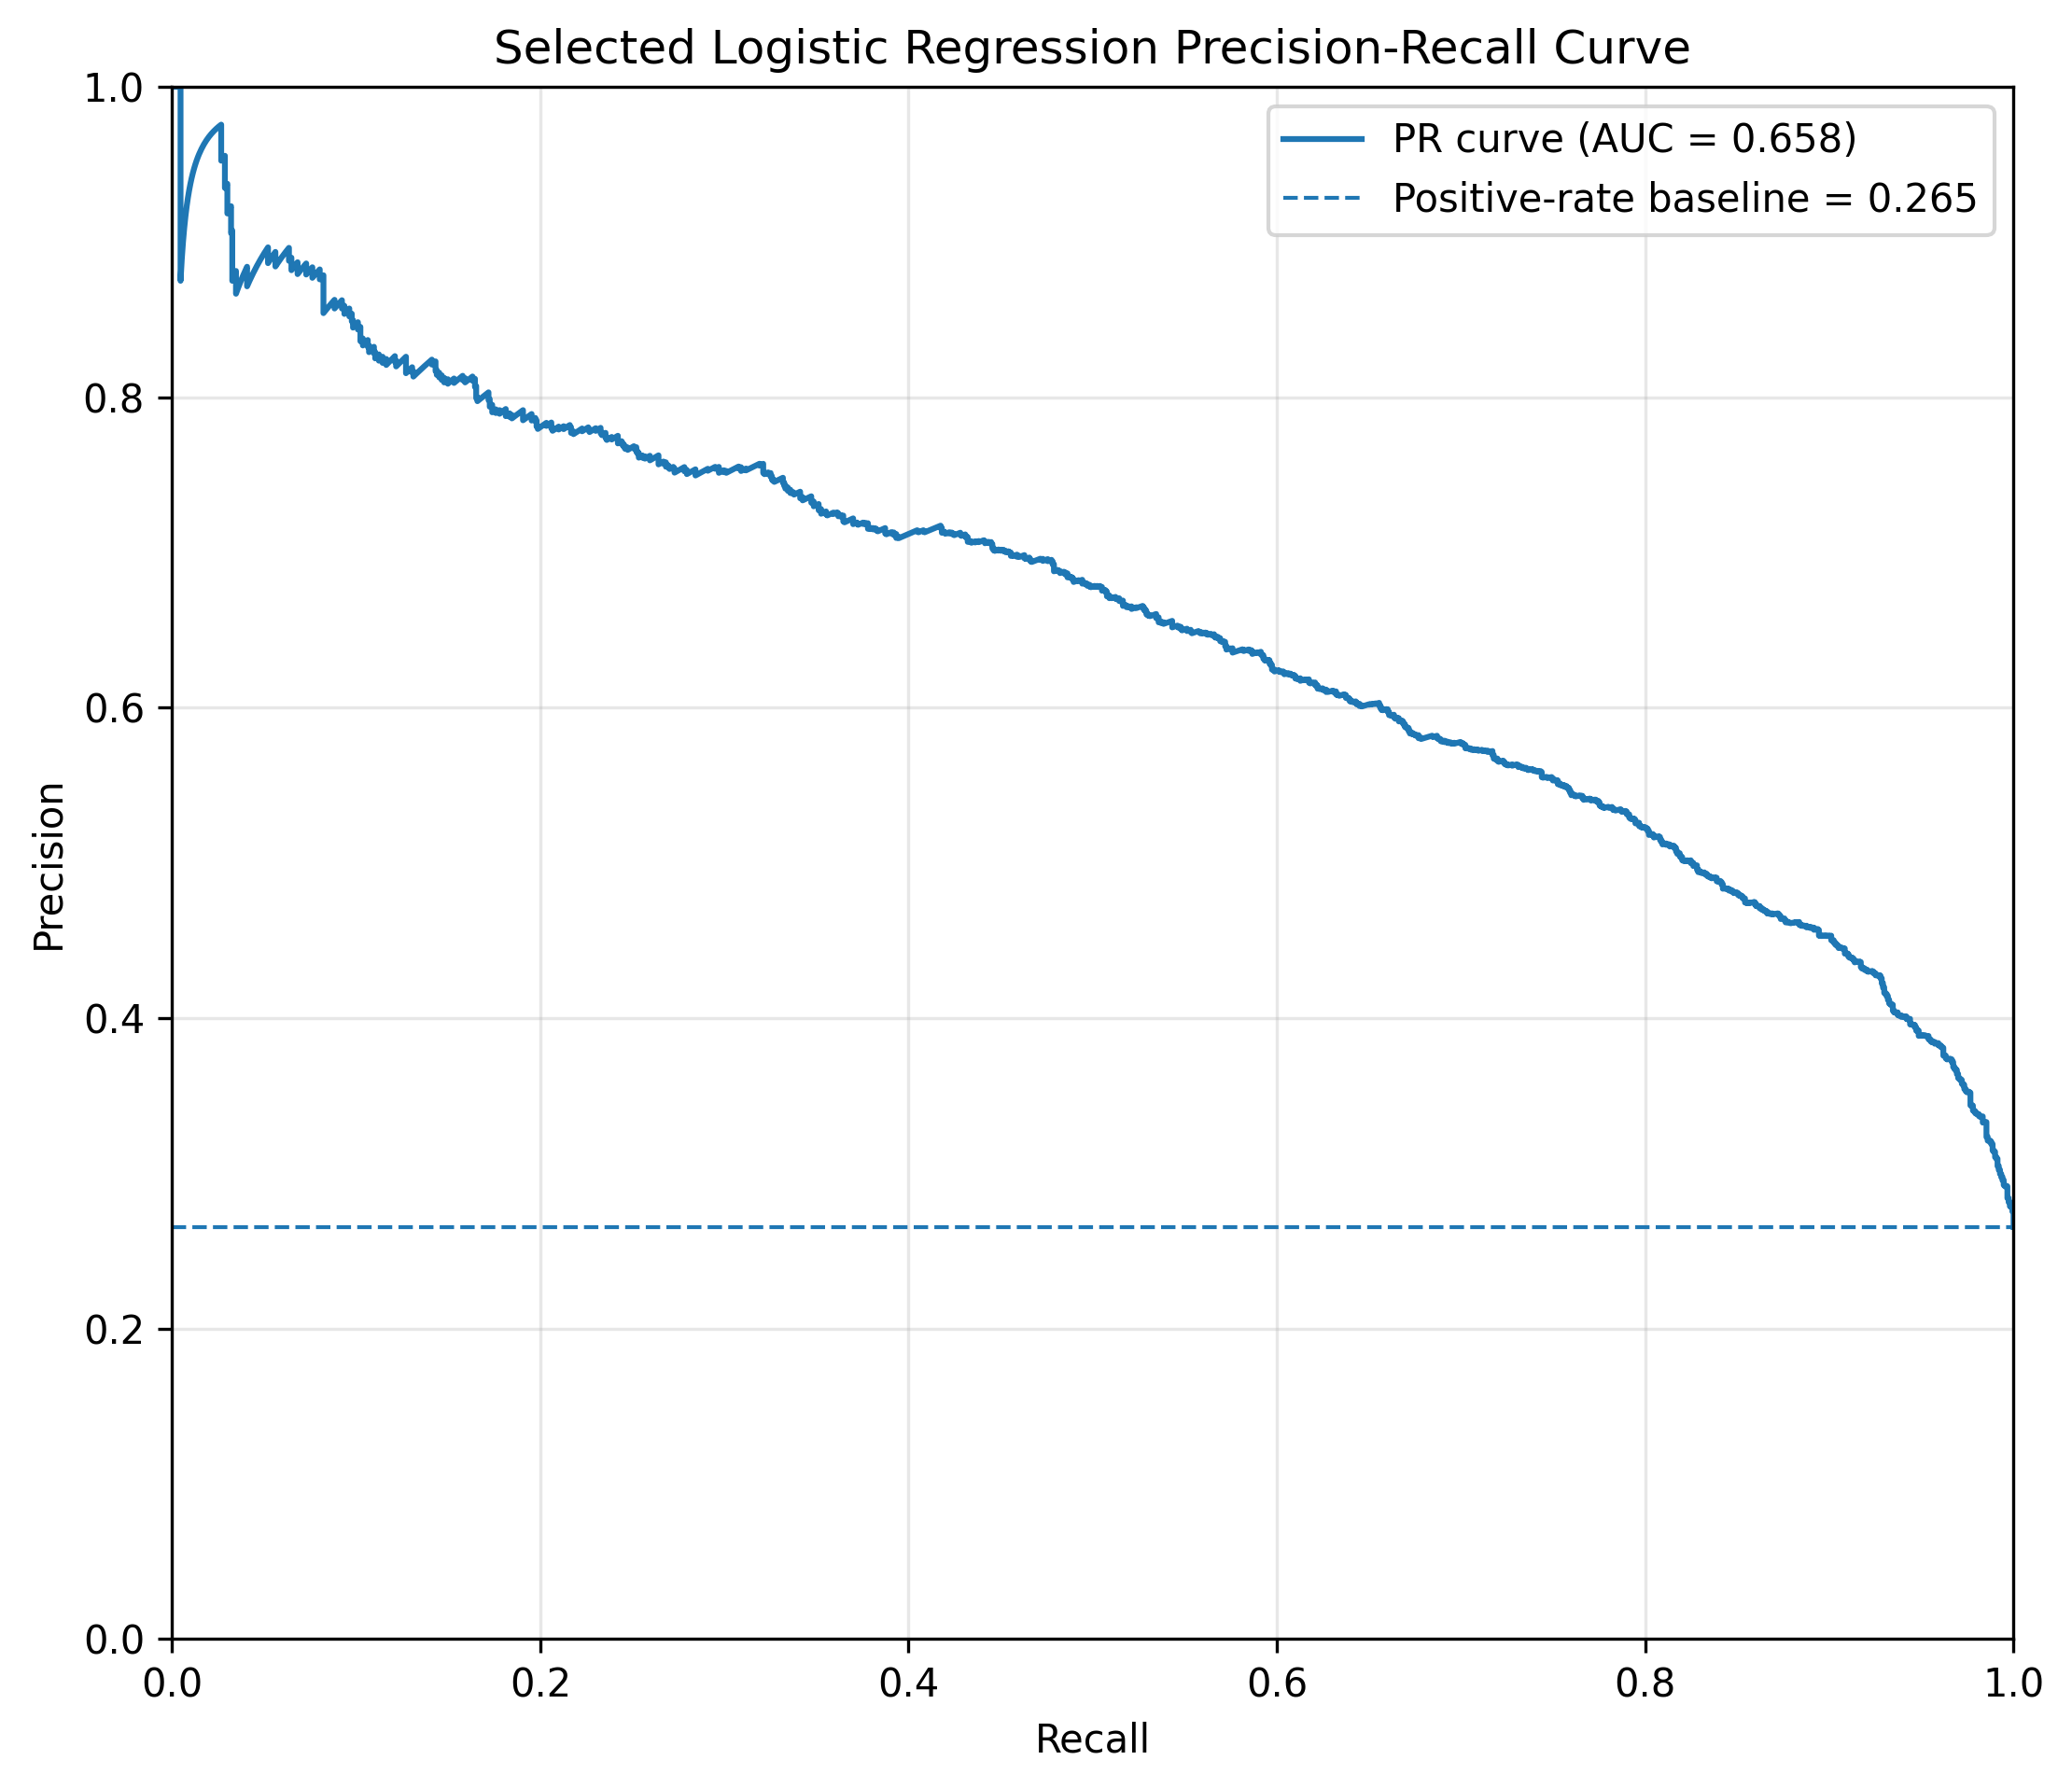
\includegraphics[width=0.76\textwidth]{../figures/logistic_precision_recall_curve.png}
\caption{Precision-recall curve for selected L2 logistic regression.}
\label{fig:logistic-pr}
\end{figure}

\subsection{Summary}

Logistic regression is a strong first learned model for the churn task. It clearly improves on non-informative baselines and provides useful probability rankings, with ROC-AUC around \(0.846\) and PR-AUC around \(0.658\). L1 and L2 regularization give very similar cross-validated performance once regularization is not excessively strong. Ridge classification is slightly weaker but remains a reasonable least-squares linear baseline.

The regularization grids show that the exact value of \(C\) is not the main conclusion. The important development-stage lesson is that extremely strong regularization underfits, while a broad moderate-to-weak regularization region performs similarly. This is why the selected L2 logistic model should be understood as a representative stable linear benchmark rather than a uniquely optimal hyperparameter setting.

The class-weighted logistic regression variant demonstrates the central classification tradeoff: it detects many more churners, but it also creates many more false positives. This confirms that model assessment cannot rely on accuracy alone. Confusion-matrix counts, recall, precision, specificity, ROC-AUC, PR-AUC, and threshold behaviour must be considered together.

The coefficient analysis is also useful. Tenure and two-year contracts are associated with lower fitted churn scores, while fiber optic internet, month-to-month contracts, and higher accumulated charges are associated with higher fitted churn scores. These patterns are consistent with the training-set EDA, but they remain predictive associations rather than causal effects.

This section establishes logistic regression as the first interpretable learned benchmark. Later model families should be compared against it by asking whether they improve ranking performance, reduce false positives at useful recall levels, or capture nonlinear feature interactions that linear models cannot represent directly. Final claims about model-family superiority are deferred to the later comparison and test-evaluation stages.
